\subsection{Präsentation von Erklärungen}
Neben dem Erstellen der Erklärung, existieren auch einige Hinweise in der wissenschaftlichen Literatur, wie diese an den Erklärungsempfänger zu übermitteln sind.
\subsubsection{Integration von Domänenwissen und Kontext}
Nach \cite{zhou20182d} ist die Integration von Domänenwissen besonders wichtig, um Erklärungen verständlicher und praxisorientierter zu gestalten. \cite{sun2005explanation} integrierten bspw. Domänenwissen in bayesche Netzwerke.

\subsubsection{Form der Präsentation}
\cite{weitz2019you} überprüfen in ihrer Veröffentlichung, ob ein virtueller Agent die von dem XAI-Algorithmus erstellten Erklärungen an Endnutzer kommunizieren könnte. Ergebnis dieser Untersuchung, dass menschliche Züge eines virtuellen Agenten die Interaktion erleichtern, was gleichzeitig zu einem besseren Verständnis und auch zu mehr Vertrauen auf Endnutzerseite führt. Hier sei jedoch angemerkt, dass Vertrauen schwer zu messen ist \cite{weitz2019you}.  Auch \cite{vaughan2020human} stellen heraus, dass für Menschen verbale sowie nonverbale Kommunikation zum Verständnis hilfreich ist.
Um für Menschen verständlichere Erklärungen generieren zu können, haben \cite{kim2020answering} eine Methode entwickelt, welche aus Charts (z.B. Balkendiagrammen) automatisch einen beschreibenden Text generieren kann.

\subsubsection{Interaktivität}
Bei der Präsentation können Visualisierungstools helfen. Interaktivität ist ein besonders wichtiges Element dieser Tools, da ein Vor- und Zurückgehen durch die Daten und Erklärungen hilfreich sein können, um die Daten und die Funktionsweise des Modells besser zu verstehen. Des Weiteren kann der Nutzer sich selbst aussuchen, was für sein Verständnis wichtig ist und wie er Informationen am besten aufnimmt \cite{vaughan2020human}. Es existieren auch Untersuchungen im wissenschaftlichen Kontext, welche die Vorteile von Interaktivität untersuchten. So fanden \cite{vaccaro2018illusion} heraus, dass Menschen mit dem Output eines System zufriedener sind, wenn sie diesen mithilfe von einem interaktiven Schieberegler abfragten. Außerdem hilft Interaktivität und die Möglichkeiten des Nutzers den Output der XAI-Methoden mitzubestimmen, dabei explorative Experimente durchzuführen \cite{weld2019challenge}. Dies erlauben beispielweise Drill-Down-Methoden hin zu konkreten Erklärungen und die Möglichkeit Erklärungen miteinander zu vergleichen oder die Wahlmöglichkeit bei den Darstellungen \cite{weld2019challenge}.

Tools können dabei helfen solche interaktiven Visualisierungsformen zu erstellen \cite{zhou20182d}. Ein solches Tool ist z.B. der Model Tracker, welcher Analysen bzgl. der Performance und Debugging ermöglicht \cite{amershi2015modeltracker}. Ein weiteres Visualisierungstool wurde von \cite{chen2016diagnostic} entwickelt, welches zehn verschiedene Techniken (shaded confusion matrix, ManiMatrix, learning curve, learning curve of multiple models, McNemar Test matrix, EnsembleMatrix, Customized SmartStripes, Customized ModelTracker, confusion matrix with sub-categories, force-directed graph) \todo{Eventuell erkläre ich diese noch oder lasse es ganz weg} zur Anwendung bereitstellt. Zur Visualisierung von Partial Dependence wurden Tools von \cite{krause2016interacting} bereitgestellt, welche sich vor allem an Data Scientists richten.

\begin{wrapfigure}{r}{0.5\textwidth}
    \centering
    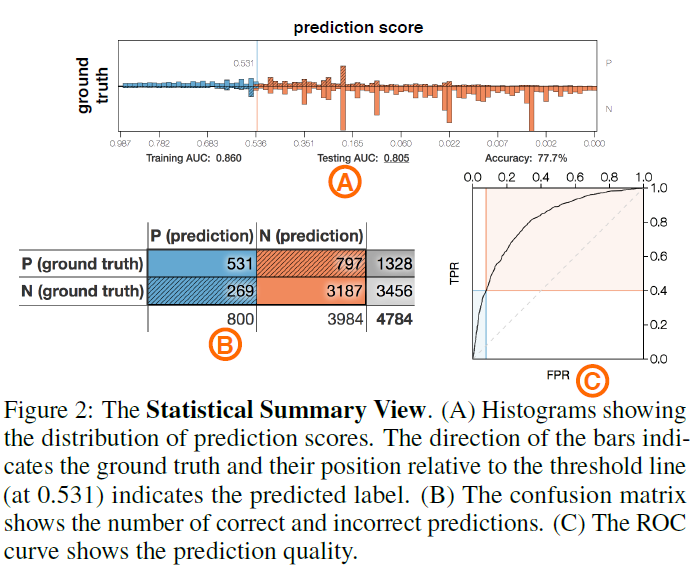
\includegraphics[scale=0.45]{pic/MA-Bilder/Literaturrecherche/25-statistsiche Summary.PNG}
    \caption{Statistische Zusammenfassung, entnommen aus \cite{krause2017workflow}}
    \label{Fig:Krause-statistischeSummary}
\end{wrapfigure}
Ein Beispiel für ein solches Tool wird an dieser Stelle kurz illustriert, um dessen Vorteile sichtbar zu machen. Der von \textcite{krause2017workflow}  entwickelte Workflow richtet sich an Domänen-Experten und Data Scientists. In ihrer Veröffentlichung wird demonstriert, wie sich durch Visualisierung ein Klassifikationsalgorithmus erklären lässt. Hierbei wird sich darauf konzentriert einzelne Instanzen zu erklären. Elemente ihrer Visualisierung sind: 
\begin{itemize}
    \item Aggregierte Statistiken verdeutlichen z.B. den Anteil korrekt und fehlerhaft klassifizierter Instanzen (vgl. Abbildung \ref{Fig:Krause-statistischeSummary})
    \item Erklärungen, welche die Relevanz einzelner Merkmale verdeutlichen
    \item Präsentation von Rohdaten, damit Nutzer diese als ergänzende Erklärungen heranziehen können
\end{itemize}
Das Prinzip des Workflows beruht auf Interaktivität, da dies die Bildung eines mentalen Modells auf Nutzerseite unterstützt und hiermit Algorithmusentscheidungen leichter nachzuvollziehen sind. Weiter abstrahieren sie von der Funktionsweise des ML-Algorithmus. Dies begründen sie darin, dass Nutzer, welche sich hiermit nicht auskennen, nur mit zu viel Wissen überfordert werden würden.
Workflow: - vorher: Erklärungen und Visualisierung (interaktiv Erklärungen für Daten anzeigen) - Outcome-Level: grundsätzliche Accuracy z.B. mit Confusion matrix - Feature-Level: Alle Erklärungen mit gleichen Merkmalen gebündelt anzeigen - Instance-Level: Erklärung für eine Instanz der Daten  Interaktive Auswahl an Erklärungen, Nutzer hat kein Zugriff auf die interen Struktur
Angewendete XAI-Methoden: Prospector [17], LIME, Martens und Provost [24 (Erklärungen für binären Input)
Grenzen des Ansatzes: nur binary-Data und kein Multihttps://de.overleaf.com/project/625d7985bac938c0561d8eda-Class
So sieht der Bums aus:
Statistische Zusammenfassung:

Explanation Explorer
\begin{figure}
    \centering
    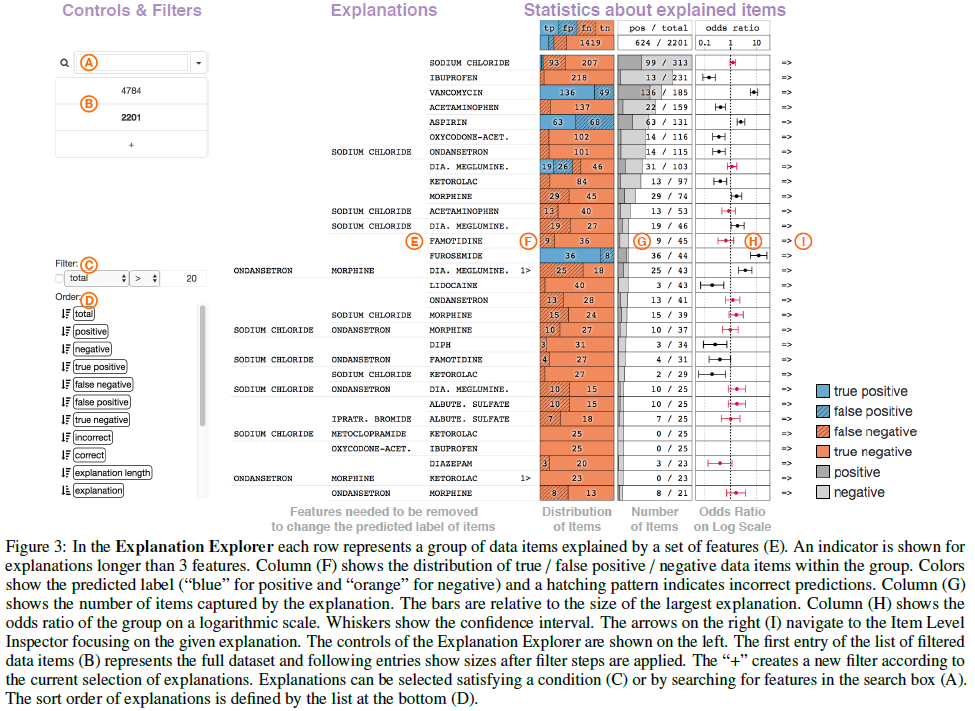
\includegraphics[scale=0.45]{pic/MA-Bilder/Literaturrecherche/25-explanationexplorer.PNG}
    \caption{explanation explorer, entommen aus: \cite{krause2017workflow}}
    \label{Fig:Krause-explanationExplorer}
\end{figure}
Itemlevel Explorer
\begin{figure}
    \centering
    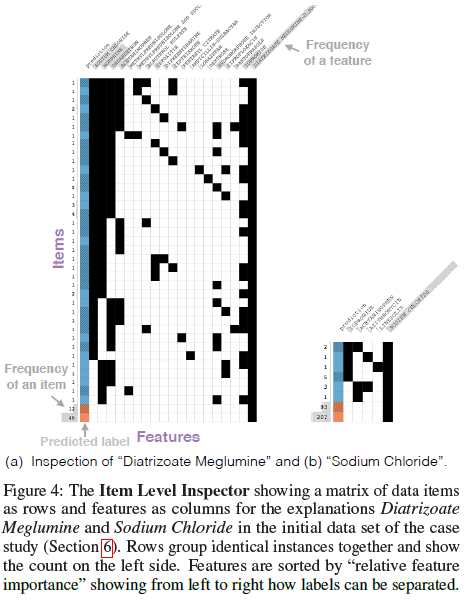
\includegraphics[scale=0.45]{pic/MA-Bilder/Literaturrecherche/25-itemlevelExplorer.PNG}
    \caption{item level explorer, entommen aus: \cite{krause2017workflow}}
    \label{Fig:Krause-itemLevelExplorer}
\end{figure}

Andere ähnliche Methoden wie die von \cite{krause2017workflow}: 
-ModelTracker [3]: Schnittstelle für Fehlererkennung und Fehlersuche bei binären Klassifizierern, die itemweise Verteilungen von Vorhersageergebnissen anzeigt. 
- Bilal et al.: confusion wheel visualization [1], um die Wahrscheinlichkeiten der Zugehörigkeit von Elementen zu verschiedenen Klassen für Mehrklassenklassifikatoren anzuzeigen. 
- Squares [26] bietet eine einzige, einheitliche Visualisierung von Leistungsmetriken und einen einfachen Zugang zu den Daten für das Debugging von Mehrklassenklassifikatoren.
- Cortez und Embrechts [9]: Ansatz der Sensitivitätsanalyse, der es den Benutzern ermöglicht, die Auswirkungen der Variation von Eingabewerten auf die Modellergebnisse zu verstehen